cd ~/%!TEX root = ../dokumentation.tex


\chapter{Implementation}\label{cha:Implementation}

\section{Lexer}\label{sec:ImplementationLexer}

As mentioned in chapter \ref{sec:ConceptLexer} the implementation of the lexer consists of the definition of tokens in form of regular expression. The following paragraph presents defined tokens and their regular expressions.

\subsubsection{Ignored symbols}
It is possible to declare certain symbol as symbol that should be ignored. However, if a symbol is declared as ignored but is specifically mentioned in another token, then if the sequence of characters represent that token, the ignored symbol is not ignored. 
In this project, tabs and white spaces are ignored as they don not have any special meaning other than providing clarity. 
Also, newlines are generally ignored because as can be seen below there are rules that cover multiple lines. If newlines wouldn't be ignored it would be difficult to ??

\begin{lstlisting}[basicstyle=\scriptsize	,caption= Example of a multi line production rule,label= lst:Lexer_example_multiline]
<annotated_formula>    ::= <thf_annotated> | <tff_annotated> | <tcf_annotated> |
                           <fof_annotated> | <cnf_annotated> | <tpi_annotated>
\end{lstlisting}

Apart from the ignored symbols, there are 13 defined tokens:

\subsubsection{Expressions}

Expressions can either grammar, token, strict or macro expression. REFERENCE
A non terminal symbol followed by the symbol itself (::=,:==,:::,...). The non terminal symbol and the symbol build a single token and are not identified as two tokens to avoid further ambiguity while parsing. Otherwise it would be difficult for the parer to determine whether the non terminal symbol that describes the rule is the start of a new rule or does still belong the previous rule because as mentioned the rules can cover multiple lines.

\textit{Regular expression of grammar expression:}  $'<\backslash w+>[\backslash s]*::='$

$\backslash w+$ matches any alphanumeric and underscore character that can occur more than one time.
$[\backslash s]*$ matches an arbitrary amount of white spaces.

\subsubsection{Non terminal symbol}

A non terminal symbol starts with \dq <\dq and ends with \dq >\dq. In between there is any arbitrary sequence of numbers, underscores and small or capital letters.

\subsubsection{Terminal symbol}

\subsubsection{Comment}

A comment is identified by the lexer as a start of a new line followed by a percentage sign followed by an arbitrary character and ends with a newline. Because the percentage sign is also part of the terminal symbols, it is necessary to check whether the percentage sign is in a newline because the terminal symbol is not because the percentage symbol when used as terminal symbol is embedded in square brackets.    

\subsubsection{Meta-Symbols}

Meta-Symbols include open and close parentheses \dq( )\dq, open and close square brackets \dq[ ]\dq, asterisks \dq *\dq and vertical bars \dq |\dq.

They are recognized by the symbol itself and have a greater meaning for the parser as they impact the to be build data structures. 

\subsubsection{Ambiguity}

The following example could either be matched as one comment token or as comment, grammar expression, non terminal symbol, terminal symbol, non terminal symbol.
This ambiguity is solved because by convention the lexer matches the longest possible token, the sequence of characters is matched as one comment.
\begin{lstlisting}[basicstyle=\scriptsize	,caption= Example of a commented out production rule,label= lst:Lexer_example]
%----   <formula_role> ::= <user_role>-<source>
\end{lstlisting}
\section{Parser}\label{sec:ImplementationParser}

The parser is taking the tokens from the lexer and matches them to defined production rules.




comment block reimplement equal operator

\subsection{Data types}\label{sec:ImplementationDataTypes}
Figure \ref{fig:ImplementationUMLExpressions} contains the UML modelling of the data types described in section \ref{sec:ConceptParserDataStructure}.
\begin{figure}[H]
\centering
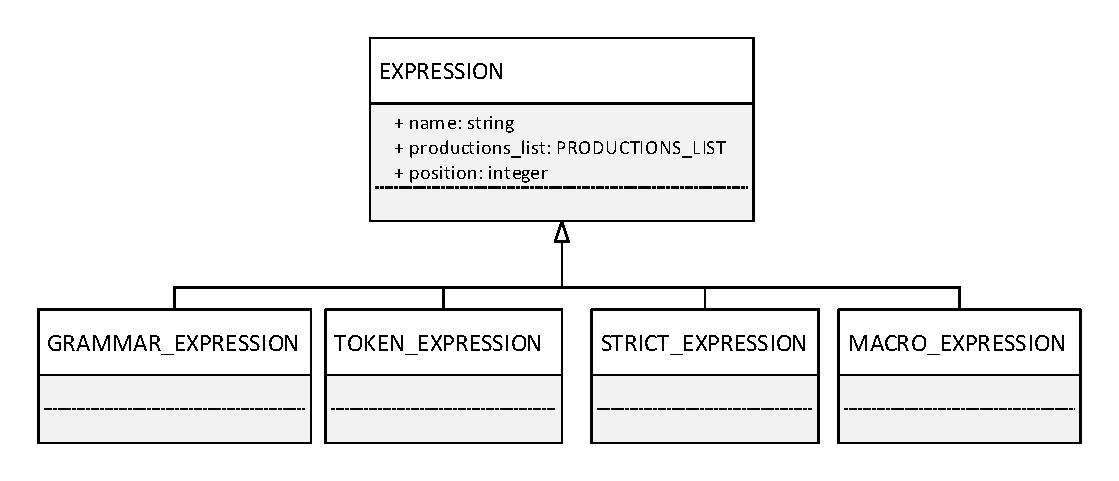
\includegraphics[width=1\textwidth]{images/uml_data_types_expressions.pdf}
\caption{UML diagram for expressions}
\label{fig:ImplementationUMLExpressions}
\end{figure}
\section{Graph generation}\label{sec:ImplementationGraphGeneration}

To generate the graph of a given grammar three algorithms are needed that will be explained in the following. 

The algorithm $buildGraphRek$ calls the function $searchProductionsListForNT$ that appends children of a node to the nodes list of children. The algorithm is first called with the start symbol. 
After the children of a node have been appended to the node, every child calls the algorithm resulting in appending their own children to their children's list. 

\begin{algorithm}[H]
\caption{Graph Generation Algorithm: buildGraphRek}
\begin{algorithmic}[1] 
\Require node
%\ENSURE $y = x^n$
\State searchProductionsListForNT(node, node.productionsList)
\If {node has children}
	\ForAll {children}
		\State buildGraphRek(child)
	\EndFor
\EndIf
\end{algorithmic}
\end{algorithm}

The right side of a production rule is stored in a productions list. For identifying the nonterminal or terminal symbols in the productions lists, a loop iterates through all elements of the productions list. Each element is a production and calls the function $searchProductionForNT$. This function identifies the children of the given element who are then appended to the node.

\begin{algorithm}[H]
\caption{Algorithm for extracting productions from productions list: searchProductionsListForNT}
\begin{algorithmic}[1] 
\Require node, productionsList
\ForAll {elements in productionsList}
	\State children = new empty list
	\State searchProductionForNT(node, element in productionsList, children)
	\State append children to node
\EndFor
\end{algorithmic}
\end{algorithm}

The goal is to identify the nonterminal symbols. Therefore it is checked if the production is a nested production and if so, the same function is called again. If the production is a XOR production list the function $searchProductionsListForNT$ is called to break down the productions list. If the production element is a nonterminal symbol the element is searched in the node dictionary to get the node where the element is on the left side. This element is then appended to a list of children. It is possible that an element appears multiple times on the left side if it is presented by multiple expressions. In this case each element is appended to the list of children.

\begin{algorithm}[H]
\caption{Algorithm for appending children to node: searchProductionForNT}
\begin{algorithmic}[1] 
\Require node, productionsElement, children
\ForAll {elements in productionsElementList}
	\If {element is  a production}
		\State {searchProductionForNT(node, element, children)}
	\ElsIf {element is a XOR productions list}
		\State {searchProductionsListForNT}
	\ElsIf {element is a nonterminal symbol}
		\State find element(s) in node dictionary
		\State append element(s) to children
	\EndIf
\EndFor
\end{algorithmic}
\end{algorithm}

\subsection{Removing of blocked productions}

Algorithm \ref{sec:remove_blocked_productions}
\begin{algorithm}[H]
\caption{Removing blocked productions}
\begin{algorithmic}[1] 
\Require control\textunderscore string
\State lines = control\textunderscore string.splitlines()
\State start\textunderscore symbol = lines[0]
\State delete lines[0]
\ForAll {line in lines}
	\State data = line.splitBy(",")
	\State nonterminal\textunderscore name = data[0]
	\State rule\textunderscore symbol = data[1]
	\State rule\textunderscore type = determineRuleType(rule\textunderscore symbol)
	\State delete data[0:2]
	\State data = parseInteger(data)
	\State data.sortReverse()
	\ForAll {index in data}
		\State node = this.nodes\textunderscore dictionary.get(Node(nonterminal\textunderscore name, rule\textunderscore type))
		\State delete node.productions\textunderscore list.list[index]
		\State delete node.children[index]
	\EndFor
\EndFor
\end{algorithmic}
\label{alg:remove_blocked_productions}
\end{algorithm}

\subsection{Determination of the remaining reachable productions}
\subsubsection{Removing non-terminating symbols}
\begin{algorithm}[H]
\caption{Removing blocked productions}
\begin{algorithmic}[1] 
\Require start\textunderscore node
\State terminating = new set()
\State temp\textunderscore terminating = new set()
\While {True}
	\State visited = new set()
	\State this.find\textunderscore non\textunderscore terminating\textunderscore symbols(start\textunderscore node, temp\textunderscore terminating, visited)
	\If {terminating == temp\textunderscore terminating}
		\State break
	\Else
		\State terminating = temp\textunderscore terminating
	\EndIf
\EndWhile
\State delete\textunderscore non\textunderscore terminating\textunderscore productions\textunderscore (start\textunderscore node, terminating, visited)
\State delete\textunderscore non\textunderscore terminating\textunderscore nodes(terminating)
\end{algorithmic}
\label{alg:remove_non_terminating_symbols}
\end{algorithm}


\section{GUI}\label{sec:GUI}
Tkinter and PyQt have been evaluated as a basis for the GUI.
-pyqt offers checkboxes in treeviews
\section{Command-line interface}\label{sec:ImplementationCommandLineInterface}
For the command-line interface (see section \ref{sec:ConceptCommandLineInterface}) the python module argparse is used.
-argparse Python offers a library for command-line interfaces.
-options for path to grammar and control file
-option for output path